\subsection{Front-end Implementering}
\label{Sec:FE-Implementering}
Til Front-end implementering er der brugt WPF med MVVM design patterns.
Til at skifte views uden at oprette et nyt vindue bruges et mediator design, hvor hver knap som skifter view giver en besked til mediatoren. Dette virker fordi alle views er oprettet som WPF user controls, og ikke views, hvilket tillader at et main view kan skifte mellem viewmodels, derved skifter vil alt indhold på vinduet, men uden at selve rammen skifter. Dette resulterer i et mere flydende User Interface for brugeren og derved en alt i alt bedre oplevelse. \cite{Mediator}\\
Et eksempel på hvordan mediatoren kaldes ved et tryk på en knap kan ses i følgende kode eksempel:

\begin{lstlisting}[language=c]
private DelegateCommand _loadGame;
    
public DelegateCommand LoadGame => _loadGame ?? (
	_loadGame = new DelegateCommand(
	ExecuteLoadCommand, CanExecuteLoadCommand));

async void ExecuteLoadCommand()
{
    await GameController.Instance.LoadGame(SelectedSave.ID);
    Mediator.Notify("GameStart", "");
}

bool CanExecuteLoadCommand()
{
    return SelectedSave != null;
}

void LoadCommand()
{
    LoadGame.RaiseCanExecuteChanged();
}
\end{lstlisting}

Visuelt er alle views implementeret tæt på det oprindelige design. Antallet og placering af knapper har ændret sig en smule, men den primære ide er uændret. Et eksempel på dette er room view.
For at se mere om hvordan andre views og menuer er implementeret se Tekniskbilag \textbf{INDSÆT REFERENCE HER}.

\subsubsection{Room View}

Visuelt er room view (\autoref{fig:Design-FE-impl-room}) ikke ændret betydeligt fra det oprindelige design. Der er ændret lidt på placering og antal af knapper så det passer til antallet af interaktioner tilgængelig til brugeren. Kortet er lavet så det  opdateres når spilleren går ind i et nyt rum, ved at ændre på synligheden af elementerne i kortet. Det er yderligere sat op så det kan skaleres til de skærmopløsninger som understøttes.\\
Ved at trykke på interact knappen kan spilleren flytte et valgt 'item' fra listen nederst til venstre over i sit inventory (et seperat view), som kan tilgås ved at trykke på Inventory knappen.\\
Alt tekst er vist med data binding.

\begin{figure}[H]
\centering
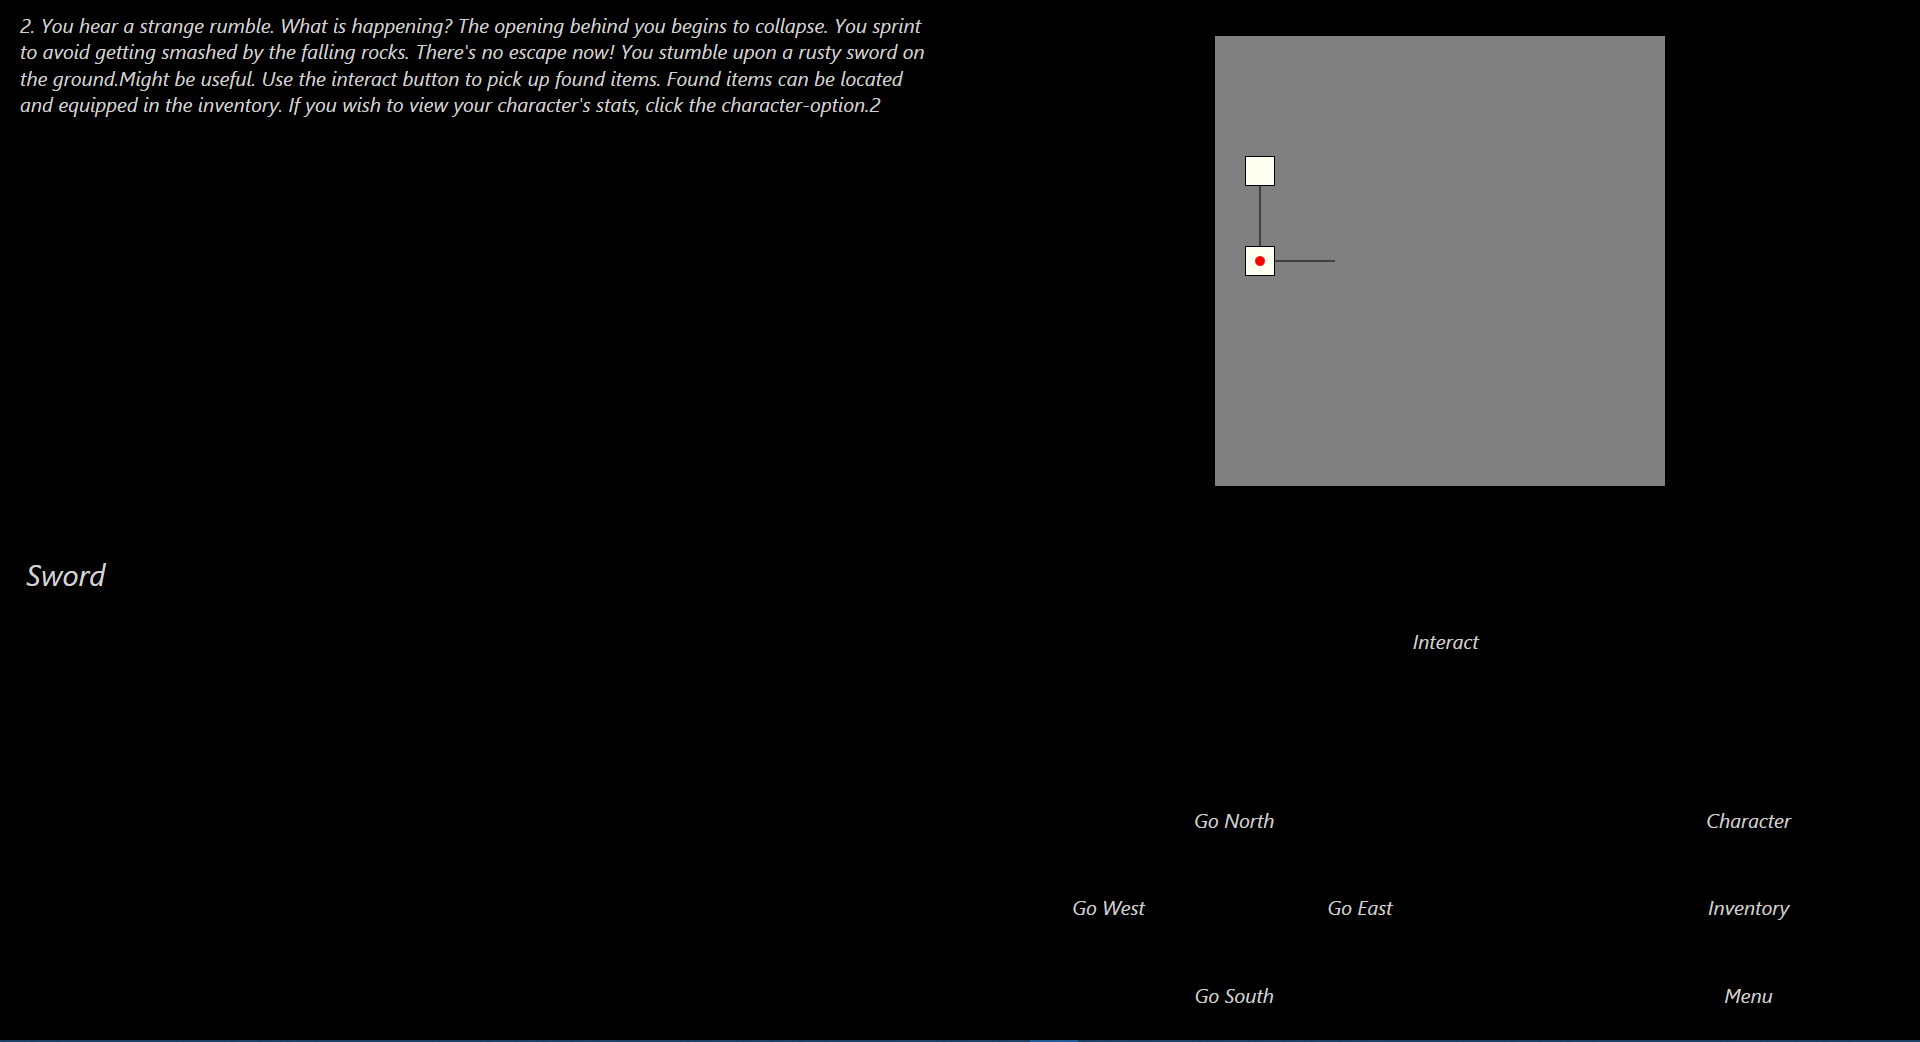
\includegraphics[width = \textwidth]{02-Body/Images/room_final.PNG}
\caption{Endeligt udseende af room view. Generelt er der ikke ændret meget i forhold til det oprindelige design. Kortet er lavet så det skalerer med skærmopløsningen.}
\label{fig:Design-FE-impl-room}
\end{figure}